\documentclass[10pt]{article}

%Math
\usepackage{amsmath}
\usepackage{amsfonts}
\usepackage{amssymb}
\usepackage{amsthm}
\usepackage{ulem}
\usepackage{stmaryrd} %f\UTF{00FC}r Blitz!

%PageStyle
\usepackage[ngerman]{babel} % deutsche Silbentrennung
\usepackage[utf8]{inputenc} 
\usepackage{fancyhdr, graphicx}
\usepackage[scaled=0.92]{helvet}
\usepackage{enumitem}
\usepackage{parskip}
\usepackage[a4paper,top=2cm]{geometry}
\setlength{\textwidth}{17cm}
\setlength{\oddsidemargin}{-0.5cm}


% Shortcommands
\newcommand{\Bold}[1]{\textbf{#1}} %Boldface
\newcommand{\Kursiv}[1]{\textit{#1}} %Italic
\newcommand{\T}[1]{\text{#1}} %Textmode
\newcommand{\Nicht}[1]{\T{\sout{$ #1 $}}} %Streicht Shit durch
\usepackage{tabto} %Möglichkeit Tabulatoren zu nutzen%

%Arrows
\newcommand{\lra}{\leftrightarrow} 
\newcommand{\ra}{\rightarrow}
\newcommand{\la}{\leftarrow}
\newcommand{\lral}{\longleftrightarrow}
\newcommand{\ral}{\longrightarrow}
\newcommand{\lal}{\longleftarrow}
\newcommand{\Lra}{\Leftrightarrow}
\newcommand{\Ra}{\Rightarrow}
\newcommand{\La}{\Leftarrow}
\newcommand{\Lral}{\Longleftrightarrow}
\newcommand{\Ral}{\Longrightarrow}
\newcommand{\Lal}{\Longleftarrow}

% Code listenings
\usepackage{color}
\usepackage{xcolor}
\usepackage{listings}
\usepackage{caption}
\DeclareCaptionFont{white}{\color{white}}
\DeclareCaptionFormat{listing}{\colorbox{gray}{\parbox{\textwidth}{#1#2#3}}}
\captionsetup[lstlisting]{format=listing,labelfont=white,textfont=white}
\lstdefinestyle{JavaStyle}{
 language=Java,
 basicstyle=\footnotesize\ttfamily, % Standardschrift
 numbers=left,               % Ort der Zeilennummern
 numberstyle=\tiny,          % Stil der Zeilennummern
 stepnumber=5,              % Abstand zwischen den Zeilennummern
 numbersep=5pt,              % Abstand der Nummern zum Text
 tabsize=2,                  % Groesse von Tabs
 extendedchars=true,         %
 breaklines=true,            % Zeilen werden Umgebrochen
 frame=b,         
 %commentstyle=\itshape\color{LightLime}, Was isch das? O_o
 %keywordstyle=\bfseries\color{DarkPurple}, und das O_o
 basicstyle=\footnotesize\ttfamily,
 stringstyle=\color[RGB]{42,0,255}\ttfamily, % Farbe der String
 keywordstyle=\color[RGB]{127,0,85}\ttfamily, % Farbe der Keywords
 commentstyle=\color[RGB]{63,127,95}\ttfamily, % Farbe des Kommentars
 showspaces=false,           % Leerzeichen anzeigen ?
 showtabs=false,             % Tabs anzeigen ?
 xleftmargin=17pt,
 framexleftmargin=17pt,
 framexrightmargin=5pt,
 framexbottommargin=4pt,
 showstringspaces=false      % Leerzeichen in Strings anzeigen ?        
}

%Config
\renewcommand{\headrulewidth}{0pt}
\setlength{\headheight}{15.2pt}

%Metadata
\fancyfoot[C]{If you use this documentation for a exam, you should offer a beer to the authors!}
\title{
	\vspace{5cm}
	Verteilte Systeme - Zusammenfassung
}
\author{Jan Fässler \& Chregi Glatthard}
\date{4. Semester (FS 2013)}


% hier beginnt das Dokument
\begin{document}

% Titelbild
\maketitle
\thispagestyle{fancy}

\newpage

% Inhaltsverzeichnis
\pagenumbering{Roman}
\tableofcontents	  	


\newpage
\setcounter{page}{1}
\pagenumbering{arabic}

% Inhalt Start

\section{Networking}
\subsection{InetAddress}
\subsubsection*{Static factory methods}
\begin{itemize}
	\item getByName(String name)
	\item getByAddress (4/16 bytes)
	\item getAllByName(String host)
	\item getLocalHost()
\end{itemize}
\subsubsection*{Instance methods}
\begin{itemize}
	\item byte[] getAddress()
	\item String getHostAddress()
	\item String getHostName()
	\item String getCanonicalHostName()
	\item boolean isReachable(int timeout)
	\item boolean isMulticastAddress()
\end{itemize}
\subsection{Network Interfaces}
\begin{lstlisting}[language=Java, caption=Network Interfaces and its addresses, style=JavaStyle]
public static void main(String[] args) throws SocketException {
	Enumeration<NetworkInterface> interfaces = NetworkInterface.getNetworkInterfaces();
	while(interfaces.hasMoreElements()){
		NetworkInterface intf = interfaces.nextElement();
		Syst	em.out.print(intf.getName());
		System.out.println(" ["+intf.getDisplayName()+"]");
		Enumeration<InetAddress> adr = intf.getInetAddresses();
		while(adr.hasMoreElements()){
			System.out.println("\t" + adr.nextElement());
		}
		byte[] hardwareAddress = intf.getHardwareAddress();
	}
}
\end{lstlisting}
\subsection{Sockets}
Abstraction through which an application may send and receive data through the network. A Socket is identified by Hostname/IP and port number.
\begin{description}
	\item[Stream Sockets] \hfill
	\begin{itemize}
		\item Use TCP as end-to-end protocol
		\item Provide a reliable byte-stream
		\item Connection oriented: Socket represents one end of a TCP connection
	\end{itemize}
	\item[Datagaram Sockets] \hfill 
	\begin{itemize}
		\item Use UDP as protocol
		\item Not connection oriented, not reliable
	\end{itemize}
\end{description}
\subsubsection{Controlling Socket Behaviors}
\begin{description}
	\item[Blocking \& Timeouts] \hfill 
	\begin{description}
		\item[ServerSocket.accept / InputStream.read] \hfill \\
			read or accept call will not block for more than a fixed number of msec otherwise, InterruptedIOException is thrown (get/setSoTimeout(int timeout))
		\item[Socket constructor] \hfill \\
			Uses a system-defined timeout, cannot be changed by Java API (Solution: use connect)
		\item[OutputStream.write] \hfill \\
			Cannot be interrupted / caused to time-out by Java API
	\end{description}
	\item[Keep-Alive] \hfill
	\begin{itemize}
		\item TCP provides a keep-alive mechanism
		\item Probe messages are sent after a certain time
		\item Application only sees keep-alive working if the probes fail!
		\item Per default keep-alive is disabled
		\item Default timeout: 2h (7200 secs)
	\end{itemize}
	\item[Send / Receive Buffer Size] \hfill
	\begin{itemize}
		\item When a Socket is created, the OS must allocate buffers to hold incoming \& outgoing data
		\item Receive buffer size may also be specified on server socket (for accepted
sockets which immediately receive data)
	\end{itemize}
	\item[No Delay] \hfill
	\begin{itemize}
		\item TCP tries to avoid sending small packets
		\item Buffers data until it has more to send, combines small packets with larger ones
		\item Necessary if application has to be efficient
		\item Default: false
	\end{itemize}
\end{description}
\subsubsection{Closing Connections}
\begin{description}
	\item[close()] \hfill 
	\begin{itemize}
		\item Once an endpoint (client or server) closes the socket, it can no longer send or receive data	
		\item Close can only be used to signal the other end that the caller is completely finished communicating
	\end{itemize}
	\item[shutdownOutput()] \hfill
	\begin{itemize}
		\item Closes output-stream, no more data can be may be written (IOException)
		\item All data written before shutdownOutput can be read by receiver
	\end{itemize}
	\item[shutdownInput()] \hfill
	\begin{itemize}
		\item Closes the input stream
		\item Any undelivered data is (silently) discarded, read operations will return -1
	\end{itemize}
	\item[s.close() / s.shutdownOutput()] \hfill
	\begin{itemize}
		\item Data may still be waiting to be delivered to the other side
		\item By default, socket tries to deliver remaining data, but if socket crashes, data may be lost without notification to sender (as close returns immediately)
	\end{itemize}
\end{description}
\subsubsection{User Datagram Protocol}
\begin{itemize}
	\item UDP allows to address applications over ports
	\item UDP adds another layer of addressing (ports) to that of IP
	\item UDP detects some form of data corruption that may occur in transit and discards corrupted messages
	\item UDP retains message boundaries
\end{itemize}

\newpage
\section{Internet}
\subsection{Protocol}
\begin{description}	
	\item[GET] \hfill
	\begin{itemize}
		\item Access of content from the server
		\item Idempotent, i.e. the side effects of N>0 identical requests is the same as for a single request ( f(f(x)) = f(x) )
	\end{itemize}
	\item[POST] \hfill \\
		Comparable to GET but Method must not necessarily be idempotent and Request data is transferred in the body of the request
	\item[HEAD] \hfill
	\begin{itemize}
		\item Identical to GET, except that the server must not return the body
		\item Can be used to request meta information (headers) about the resource
	\end{itemize}
	\item[OPTIONS (1.1)] \hfill \\
		Returns information about the communication options available on the specified resource (or on the server in general if request URI=*)
	\item[PUT (1.1)] \hfill \\
		Stores a web page on the server (rarely implemented)
	\item[DELETE (1.1)] \hfill \\
		Removes a web resource from the servver (rarely implemented)
	\item[TRACE (1.1)] \hfill \\
		Returns the request as it was accepted by server ($\Ra$ debugging)
	\item[CONNECT (1.1)] \hfill \\
		Implemented by Proxy Server capable to provide an SSL tunnel
\end{description}
\subsubsection{Response Codes}
\begin{description}
	\item[200-299: Success] \hfill
	\begin{itemize}
		\item[200] OK
		\item[201] Created
		\item[202] Accepted
	\end{itemize}
	\item[300-399: Redirections] \hfill
	\begin{itemize}
		\item[300] Multiple Choices
		\item[301] Moved Permanently
		\item[302] Found
		\item[303] See Other (e.g. after POST)
		\item[304] Not Modified
		\item[305] Use Proxy
		\item[307] Temporary Redirect
	\end{itemize}
	\item[400-499: Client Error] \hfill
	\begin{itemize}
		\item[400] Bad Request
		\item[401] Unauthorized
		\item[402] Payment Required
		\item[403] Forbidden
		\item[404] Not Found
		\item[405] Method Not Allowed
		\item[407] Proxy Authentication Required
		\item[408] Request Time-out
		\item[411] Length Required
		\item[413] Request Entity Too Large
		\item[414] Request-URI Too Large
		\item[415] Unsupported Media Type
	\end{itemize}
	\item[500-599: Server Error] \hfill
	\begin{itemize}
		\item[500] Internal Server Error
		\item[501] Not Implemented
		\item[503] Service Unavailable
		\item[505] HTTP Version not supported
	\end{itemize}
\end{description}
\subsection{Request Headers}
\begin{description}
	\item[Host] server host 
	\item[Referer] host from which the request is initiated
	\item[Accept] data types supported by the client 
	\item[Accept-Language] language supported by client
	\item[Accept-Encoding] encodings supported by client, e.g. gzip or deflate
	\item[User-Agent] browser details, supplies server with information about the type of browser making the request
	\item[Connection: Keep-Alive] browser is requesting the use of persistent TCP connections
\end{description}
\subsection{Response Headers}
\begin{description}
	\item[Content-Type] MIME-Type of content
	\item[Content-Length] size of body (in bytes)
	\item[Content-Encoding] compression algorithms
	\item[Location] used by redirections
	\item[Date] timestamp when the response was created 
	\item[Last-Modified] modification date of resource (assumed by server) 
	\item[Expires] date after which the result is considered stale 
	\item[Server] information about the server
	\item[Transfer-Encoding] specifies type of transformation
	\item[Cache-Control] information about cache handling (e.g. no-cache disables caching)
	\item[WWW-Authenticate] information about authentication method
\end{description}
\subsection{Servlet}
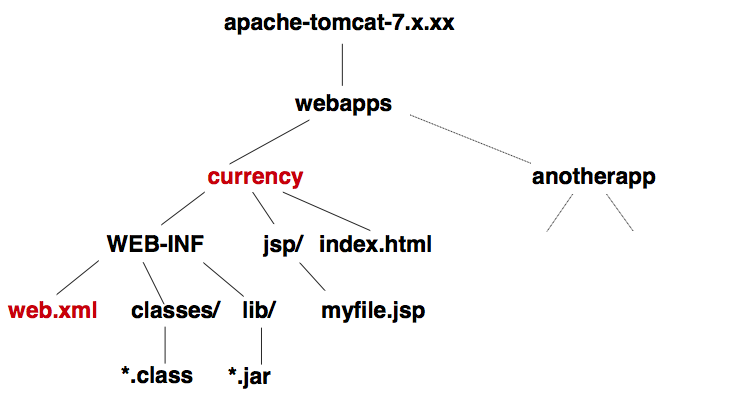
\includegraphics[scale=0.5]{tomcat-structure.png}
\begin{lstlisting}[language=Java, caption=Servlet Example, style=JavaStyle]
public class Converter extends HttpServlet {
	public void doGet(HttpServletRequest request, HttpServletResponse response) throws IOException {
		response.setContentType("text/html");
		PrintWriter out = response.getWriter();
		String amount = request.getParameter("amt"); 
		String from = request.getParameter("from"); 
		String to = request.getParameter("to"); 
		String res = computeResult(amount, from, to);
		out.println("<html>\n<body bgcolor=\"white\">"); 
		out.println("<h1>Currency Converter</h1>"); 
		out.println(amount + " " + from + " = " + res);
		out.println("</body>\n</html>");
	}
	String computeResult(String amount, String from, String to){...}
}
\end{lstlisting}
\begin{lstlisting}[language=Java, caption=web.xml, style=JavaStyle]
<?xml version="1.0" encoding="ISO-8859-1"?>
<web-app xmlns="http://java.sun.com/xml/ns/javaee" xmlns:xsi="http://www.w3.org/2001/XMLSchema-instance" xsi:schemaLocation="http://java.sun.com/xml/ns/javaee http://java.sun.com/xml/ns/javaee/web-app_3_0.xsd" version="3.0">
    <servlet>
        <servlet-name>CurrencyConverter</servlet-name>
        <servlet-class>ch.fhnw.ds.Converter</servlet-class>
    </servlet>
    <servlet-mapping>
        <servlet-name>CurrencyConverter</servlet-name>
		<url-pattern>/convert</url-pattern>
	</servlet-mapping>
</web-app>
\end{lstlisting}

\newpage
\section{Webservices}
\subsection{XML-RPC}

simples RPC Protokoll über HTTP, benötigt keine lange Einarbeitungszeit
\subsubsection{Primitive Datentypen}
\begin{itemize}
\item int, i4 \tab signed 32bit Integer
\item string \tab ASCII string (no latin1)
\item boolean \tab either 0 or 1
\item double \tab double-precision floating point number
\item dateTime.iso8601 \tab z.B. 20050717T14:08:14
\item base64 \tab raw binary data, base64 encoded
\end{itemize}

\begin{lstlisting}[language=Java, caption=Beispiele, style=JavaStyle]
<i4>13</i4>
<boolean>0</boolean>
\end{lstlisting}

\subsubsection{Structs}
\begin{itemize}
\item Struct enthält Members mit Name und Wert.
\item können rekursiv sein (Structs die Structs enthalten)
\end{itemize}

\begin{lstlisting}[language=Java, caption=Struct Beispiel, style=JavaStyle]
<i4>13</i4>
<struct> 
  <member> 
    <name>from</name> 
    <value><i4>-5</i4></value> 
  </member> 
  <member> 
    <name>to</name> 
    <value><i4>5</i4></value> 
  </member>
</struct>
\end{lstlisting}

\subsubsection{Arrays}
\begin{itemize}
\item Element-Typen können gemischt werden
\end{itemize}

\begin{lstlisting}[language=Java, caption=Array, style=JavaStyle]
<array>
 <data>
  <value><i4>-5</i4></value>
  <value><string>44</string></value>
  <value><boolean>1</boolean></value>
 </data> 
</array>
\end{lstlisting}

\subsubsection{XML-RPC Request}
\begin{lstlisting}[language=Java, caption=Method Call, style=JavaStyle]
<?xml version="1.0" encoding="UTF-8"?>
<methodCall>
  <methodName>Echo.getEcho</methodName>
    <params>
      <param>
        <value>World</value>
      </param>
    </params>
</methodCall>
\end{lstlisting}

\subsubsection{XML-RPC Response}
\begin{lstlisting}[language=Java, caption=Single Result, style=JavaStyle]
<?xml version="1.0" encoding="UTF-8"?>
<methodResponse>
  <params>
    <param>
      <value>Hello World, welcome to XML-RPC</value>
    </param>
  </params>
</methodResponse>
\end{lstlisting}
Als Resultat kann nur ein Wert zurückkommen, dieser kann jedoch auch ein Struct oder ein Array sein.

\begin{lstlisting}[language=Java, caption=Fault Result, style=JavaStyle]
<?xml version="1.0" encoding="UTF-8"?>
<methodResponse>
  <fault>
    <value>
      <struct>
        <member>
          <name>faultCode</name>
          <value><i4>0</i4></value>
        </member>
        <member>
          <name>faultString</name>
          <value>No such handler: Echo.foo</value>
        </member>
      </struct>
    </value>
  </fault>
</methodResponse>
\end{lstlisting}

\subsubsection{Apache XML-RPC Sample Server}
\lstinputlisting[language=java,caption=Sample Server,style=JavaStyle]{code/ApacheXML-RPC-Server1.class}

\lstinputlisting[language=java,caption=Handler Class Server,style=JavaStyle]{code/ApacheXML-RPC-Server2.class}

Nur Instanzmethoden der Handlerklasse sind zugreifbar. Keine void Methoden. Public Default Constructor zwingend.

\subsubsection{Apache XML-RPC Client}
\lstinputlisting[language=java,caption=Handler Class Server,style=JavaStyle]{code/ApacheXML-RPC-Client.class}


\subsection{SOAP}
\subsubsection{WSDL (Web Services Description Language)}
(früher Web Services Definition Language)\linebreak
WSDL ist eine XML basierte Interface Beschreibungssprache die genutzt wird um die Funktionalität von Webservices zu beschreiben. Eine WSDL Beschreibung eines Webservices enthält:
\begin{itemize}
\item Wie der Service aufgerufen werden kann
\item Welche Parameter er erwartet
\item Welche Datenstruktur er zurückgibt
\end{itemize}

\subsubsection{JAX-WS (Java API for XML Web Services}
JAX-WS ist eine Java API um Webservices zu erstellen. Es ist Teil der Java EE (Enterprise Edition) Plattform von Sun Microsystems. Wie auch andere Java EE APIs nutzt JAX-WS Annotationen (@Webservice, @WebMethod usw). Basiert auf SOAP. Nur WSDL 1.1 unterstützt.

\subsubsection{Anleitung JAX-WS}
1. Interface erstellen
\begin{lstlisting}[language=Java, caption=Interface erstellen, style=JavaStyle]
package ch.fhnw.ds.jaxws.server;
import javax.jws.WebService;
@WebService
public interface HelloService {
	String sayHello(@WebParam(name = "name") String name);
}
\end{lstlisting}

2. Interface implementieren
\begin{lstlisting}[language=Java, caption=Interface implementieren, style=JavaStyle]
package ch.fhnw.ds.jaxws.server; 
import java.util.Date; 
@WebService 
public class HelloServiceImpl implements HelloService { 
	@Override 
	public String sayHello(@WebParam(name = "name") String name){ 
		return "Hello " + name + " from SOAP at " + new Date(); 
	} 
}
\end{lstlisting}
3. Java Objekte für XML Requests \& Responses generieren
\% wsgen -cp bin -keep -s src -d bin ch.fhnw.ds.jaxws.server.HelloServiceImpl
\begin{itemize}
\item cp <path> classpath
\item keep keep generated files
\item s <path> path where to place generated source files
\item d <path> path where to place generated output files
\item <SEI> specify a SIB (service implementation bean)
\end{itemize}
\begin{lstlisting}[language=Java, caption=SayHello, style=JavaStyle]
package ch.fhnw.ds.jaxws.server.jaxws;
import ...;
@XmlRootElement(name = "sayHello", 
		namespace = "http://server.jaxws.ds.fhnw.ch/")
@XmlAccessorType(XmlAccessType.FIELD)
@XmlType(name = "sayHello",
		namespace = "http://server.jaxws.ds.fhnw.ch/")
public class SayHello {

	@XmlElement(name = "name", namespace = "")
	private String name;
	public String getName() { return this.name; }
	public void setName(String name) { this.name = name; }
}

\end{lstlisting}
\begin{lstlisting}[language=Java, caption=SayHelloResponse, style=JavaStyle]
package ch.fhnw.ds.jaxws.server.jaxws;
import ...;
@XmlRootElement(name = "sayHelloResponse",
		namespace = "http://server.jaxws.ds.fhnw.ch/")
@XmlAccessorType(XmlAccessType.FIELD)
@XmlType(name = "sayHelloResponse",
		namespace = "http://server.jaxws.ds.fhnw.ch/")
public class SayHelloResponse {

	@XmlElement(name = "return", namespace = "")
	private String _return;
	public String getReturn() { return this._return; }
	public void setReturn(String _return) {
		this._return = _return;
	}
}
\end{lstlisting}
4. Service publishen
\begin{lstlisting}[language=Java, caption=HelloServicePublisher, style=JavaStyle]
package ch.fhnw.ds.jaxws.server;
import javax.xml.ws.Endpoint;

public class HelloServicePublisher {
	public static void main(String[] args){
		Endpoint.publish(
			"http://127.0.0.1:9876/hs", // publication URI
			new HelloServiceImpl()); // SIB instance
		System.out.println("service published");
	}
}
\end{lstlisting}

5. Generierte Webservice Definition anschauen
http://localhost:9876/hs?wsdl
\begin{lstlisting}[language=Java, caption=WSDL, style=JavaStyle]
<?xml version="1.0" encoding="UTF-8"?> <definitions 	xmlns:soap="http://schemas.xmlsoap.org/wsdl/soap/" 	xmlns:tns="http://server.jaxws.ds.fhnw.ch/" 	xmlns:xsd="http://www.w3.org/2001/XMLSchema" 	xmlns="http://schemas.xmlsoap.org/wsdl/" 	targetNamespace="http://server.jaxws.ds.fhnw.ch/" 	name="HelloServiceImplService"> 
<types> 
	<xsd:schema> 
		<xsd:import namespace="http://server.jaxws.ds.fhnw.ch/" schemaLocation="http://localhost:9876/hs?xsd=1"> 
		</xsd:import> 
	</xsd:schema> 
</types>
<message name="sayHello">
<part name="parameters"
element="tns:sayHello">
</part>
</message>
<message name="sayHelloResponse">
<part name="parameters"
element="tns:sayHelloResponse">
</part>
</message>
<portType name="HelloServiceImpl">
<operation name="sayHello">
<input message="tns:sayHello"></input>
<output message="tns:sayHelloResponse"></output>
</operation>
</portType>
<binding name="HelloServiceImplPortBinding" 
type="tns:HelloServiceImpl"> 
<soap:binding 
transport="http://schemas.xmlsoap.org/soap/http" 
style="document"> 
</soap:binding> 
<operation name="sayHello"> 
<soap:operation soapAction=""></soap:operation> 
<input> 
<soap:body use="literal"></soap:body> 
</input> 
<output> 
<soap:body use="literal"></soap:body> 
</output> 
</operation> 
</binding>
<service name="HelloServiceImplService">
<port name="HelloServiceImplPort"
binding="tns:HelloServiceImplPortBinding">
<soap:address location="http://localhost:9876/hs">
</soap:address>
</port>
</service>
</definitions>

Referenzierte Schema Definition:

<?xml version="1.0" encoding="UTF-8"?>
<xs:schema xmlns:tns="http://server.jaxws.ds.fhnw.ch/" xmlns:xs="http://www.w3.org/2001/XMLSchema"
version="1.0"
targetNamespace="http://server.jaxws.ds.fhnw.ch/">
<xs:element name="sayHello" type="tns:sayHello"></xs:element> <xs:element name="sayHelloResponse" type="tns:sayHelloResponse"></xs:element> 
<xs:complexType name="sayHello">
  <xs:sequence> 
    <xs:element name="name" type="xs:string" minOccurs="0"></xs:element> 
  </xs:sequence> 
</xs:complexType> 
<xs:complexType name="sayHelloResponse"> 
  <xs:sequence> 
    <xs:element name="return" type="xs:string" minOccurs="0"></xs:element> 
  </xs:sequence>
 </xs:complexType> 
</xs:schema>

\end{lstlisting}

6. Client Proxy generieren
\% wsimport -keep -p ch.fhnw.ds.jaxws.client.jaxws -d bin -s src 
\begin{itemize}
\item -keep keep generated files
\item -p <package> specify (overwrite) target package
\item -s <path> path where to place generated source files
\item -d <path> path where to place generated output files
\item <WSDL> Web Service Definition
\item => HelloServiceImpl generated interface
\item => HelloServiceImplService factory class
\end{itemize}


7. Client Applikation schreiben
\begin{lstlisting}[language=Java, caption=Client, style=JavaStyle]
package ch.fhnw.imvs.client;
import ch.fhnw.imvs.client.jaxws.HelloServiceImpl;
import ch.fhnw.imvs.client.jaxws.HelloServiceImplService;

public class Client {
	public static void main(String[] args) {
		HelloServiceImplService service =
			new HelloServiceImplService();
		HelloServiceImpl port =
			service.getHelloServiceImplPort();
		String result = port.sayHello("Dominik");
		System.out.println(result);
	}
}
\end{lstlisting}

8. JAX-WS HTTP Request
\begin{lstlisting}[language=Java, caption=..., style=JavaStyle]
POST /hs HTTP/1.1						HTTP Request
Accept: text/xml, multipart/related
User-Agent: JAX-WS RI 2.2.4-b01
Host: 127.0.0.1:9877
Connection: keep-alive
Content-Length: 209
Content-Type: text/xml; charset=utf-8		SOAP HTTP Binding
SOAPAction: "http://server.jaxws.ds.fhnw.ch/HelloServiceImpl/sayHelloRequest"

<?xml version="1.0" ?>					SOAP Payload
<S:Envelope xmlns:S="http://schemas.xmlsoap.org/soap/envelope/">
	<S:Body>
		<ns2:sayHello xmlns:ns2="http://server.jaxws.ds.fhnw.ch/">
			<name>Dominik</name>
		</ns2:sayHello>
	</S:Body>
</S:Envelope>


\end{lstlisting}
9. JAX-WS HTTP Response
\begin{lstlisting}[language=Java, caption=..., style=JavaStyle]
HTTP/1.1 200 OK						HTTP Response
Transfer-encoding: chunked
Content-type: text/xml; charset=utf-8
Date: Mon, 18 Mar 2013 00:06:44 GMT
Content-Length: 277

<?xml version="1.0" ?>					SOAP Payload
<S:Envelope xmlns:S="http://schemas.xmlsoap.org/soap/envelope/">
<S:Body>
<ns2:sayHelloResponse
xmlns:ns2="http://server.jaxws.ds.fhnw.ch/">
<return>
Hello Dominik from SOAP at Mon Mar 18 01:06:44 CET 2013
</return>
</ns2:sayHelloResponse>
</S:Body>
</S:Envelope>

\end{lstlisting}

\subsection{Vergleich SOAP und XML-RPC}
\begin{tabular}{|c|c|c|}
\hline 
Feature & XML-RPC & SOAP \\ 
\hline
Structs & yes & yes \\ 
\hline 
Arrays & yes & yes \\ 
\hline 
Named structs \& arrays & no & yes \\ 
\hline 
Short learning curve & yes & no \\ 
\hline 
Developer specified character set & no & yes \\ 
\hline 
Developer defined data types & no & yes \\ 
\hline 
Can specify recipient & no & yes \\ 
\hline 
Require client understanding & no & yes \\ 
\hline 
Message specific processing instructions & no & yes \\ 
\hline  
\end{tabular} 

\newpage
\section{Representation State Transfer (REST)}
\subsection{Prinzipien}
\begin{itemize}
	\item Addressability - Give everything an ID
	\item Uniform, Constrained Interface
	\item Representation-oriented
	\item Link things together - Use Resource references
	\item Stateless communications - Resources hold state
	\item Use standard HTTP methods
\end{itemize}
\subsubsection{Addressability}
\begin{itemize}
	\item Resources = key abstractions in REST
	\item Each resource is addressable via a URI
\end{itemize}
\begin{lstlisting}[language=Java, caption=REST example, style=JavaStyle]
http://www.example.com/customers/1234 http://www.example.com/customers?lastName=Meier http://www.example.com/orders/2011/03/445245 http://www.example.com/products/ http://www.example.com/products/4711
\end{lstlisting}
\subsubsection{CRUD}
\begin{description}
	\item[READ] \hfill
	\begin{itemize}
		\item HTML: \textbf{GET, HEAD}
		\item Retrieve information in a particular representation
		\item No side effects, possibly cached
		\item May contain query parameters
	\end{itemize}
	\item[CREATE] \hfill
	\begin{itemize}
		\item HTML: \textbf{POST}
		\item Create a new sub-resource (without known ID)
	\end{itemize}
	\item[CREATE \& UPDATE] \hfill
	\begin{itemize}
		\item HTML: \textbf{PUT}
		\item Update an existing resource
		\item Create a new resource with a known ID
	\end{itemize}
	\item[DELETE] \hfill
	\begin{itemize}
		\item HTML: \textbf{DELETE}
		\item Remove resources
	\end{itemize}
	\item[OPTIONS] \hfill \\
	Returns allowed operations
\end{description}
\subsubsection{Representation-oriented}
Allow multiple representations of a resource: 
\begin{itemize}
	\item text/html
	\item text/plain
	\item application/json
	\item application/xml
\end{itemize}
\subsubsection{Link things together}
References to other resources may be used in representations
\begin{lstlisting}[language=Java, caption=example, style=JavaStyle]
<order>
   <date>16.03.2013</date>
   <amount>23</amount>
   <product ref="http://example.com/products/4711" />
   <customer ref="http://example.com/customers/1234" />
</order>
\end{lstlisting}

\subsection{SOAP vs REST}
\begin{tabular}{l | l}
	\textbf{REST} & \textbf{SOAP} \\
	\hline
	Resource Oriented & Service oriented \\
	Messages represented in different formats & Messages represented in XML \\
	HTTP used as protocol & Can be bound to different protocols \\
	HTTP verbs are used for access and manipulation & Access and Manipulation is service specific \\
	HTTP error codes are used as error messages & Fault Elements in SOAP body describes errors \\
	No formal interface description language & WSDL is used as interface description language \\
	GET requests can be cached in a proxy & All requests are POST requests, no caching!
\end{tabular}
\begin{center}
	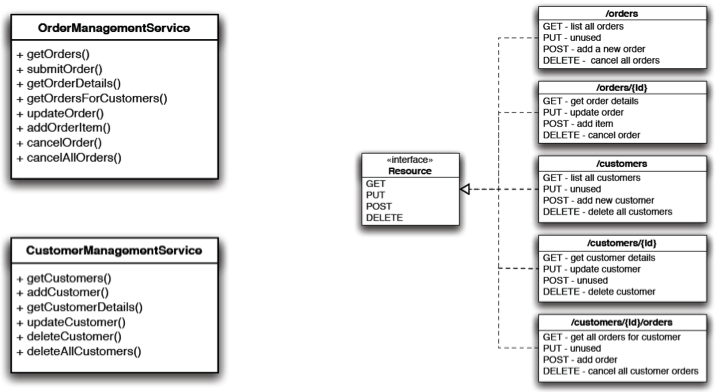
\includegraphics[scale=0.5]{soap-rest.png}
\end{center}

\subsection{JAX-RS}
\subsubsection{HTTP Methods}
\begin{itemize}
	\item Annotate resource class methods with HTTP method annotations @GET, @POST, @PUT, @DELETE, @HEAD
	\item Java method name has no significance
	\item Return value is mapped to the response (void = no response)
\end{itemize}

\begin{lstlisting}[language=Java, caption=JAX-RS Service = Annotated Java Class, style=JavaStyle]
@Singleton
@Path("/polls")
public class DoodlePoolResource {
	@GET
	@Path("{id}")
	public String getPoll(@PathParam("id") String key){ ... }
	
	@PUT
	@Path("{id}")
	public String putPoll(@PathParam("id") String key){ ... }
	
	@DELETE
	@Path("{id}")
	public void deletePoll(@PathParam("id") String key){ ... }
}
\end{lstlisting}
\subsubsection{Injection}
\begin{itemize}
	\item Automatic Type Conversion from Strings to
	\begin{itemize}
		\item Primitive types (int, short, float, double, byte, char, boolean)
		\item Classes T which have a constructor with a single String parameter
		\item Classes T which contain a static method T valueOf(String arg)
	\end{itemize}
	\item Default values may be defined with @DefaultValue for the case that the parameter is not passed with the request
\end{itemize}
\begin{description}
	\item[PathParam] \hfill \\
		Allows to extract values from URI template parameters
	\item[MatrixParam] \hfill \\
		Allows to extract matrix parameters ( /images/cars;color=blue/2010/)
	\item[QueryParam] \hfill \\
		Allows to extract query parameters added to a URI
	\item[FormParam] \hfill \\
		Allows to extract values from posted form data
	\item[HeaderParam] \hfill \\
		Allows to extract request headers
	\item[CookieParam] \hfill \\
		Allows to extract values from HTTP cookies
\end{description}
\subsubsection{Content Negotiation}
\begin{description}
	\item[@Produces] declares type of result, default: all types are supported \\
		@Produces(\{"{}text/plain", "{}text/html"\})
	\item[@Consumes] declares type which is accepted (PUT / POST) \\
		@Consumes("{}application/x-www-form-urlencoded")
\end{description}
\subsection{Data Binding}
\begin{lstlisting}[language=Java, caption=XStream Provider, style=JavaStyle]
@Provider
@Consumes("application/xstream")
@Produces("application/xstream")
public class XStreamProvider implements MessageBodyReader<Object>, MessageBodyWriter<Object>{
	private XStream xstream = new XStream(new DomDriver());
	
	public boolean isReadable(Class<?> type, Type genericType, Annotation[] annotations, MediaType mimeType) {
		return true;
	}
	public Object readFrom(Class<Object> type, Type genericType, Annotation[] annotations, MediaType mimeType, MultivaluedMap<String, String> httpHeaders, InputStream entityStream) {
		return xstream.fromXML(entityStream);
	}
	public boolean isWriteable(Class<?> type, Type genericType, Annotation[] ann, MediaType mimeType) {
		return true;
	}
	
	public long getSize(Object object, Class<?> type, Type genericType, Annotation[] ann, MediaType mimeType) {
		return -1;// size not yet known
	}
	
	public void writeTo(Object object, Class<?> type, Type genericType, Annotation[] ann, MediaType mimeType, MultivaluedMap<String, Object> httpHeaders, OutputStream entityStream) {
		xstream.toXML(object, entityStream);
	}
}
\end{lstlisting}
\begin{lstlisting}[language=Java, caption=XStream Example, style=JavaStyle]
public class Client {
	public static void main(String[] args) {
	ClientConfig config = new DefaultClientConfig();
	config.getClasses().add(XStreamProvider.class);
	Client c = Client.create(config);
	WebResource r = c.resource("http://localhost:9998/msg");
	Msg msg = new Msg("Hello from XClient");
	r.type("application/xstream").put(msg);
	Msg res = r.accept("application/xstream").get(Msg.class); 
	System.out.println(res);
	System.out.println(res.getText());
	System.out.println(res.getDate());
	}
}
\end{lstlisting}
\subsection{JAXB}
Java Architecture for XML Binding, kurz JAXB, ist eine Programmschnittstelle in Java, die es ermöglicht, Daten aus einer XML-Schema-Instanz heraus automatisch an Java-Klassen zu binden, und diese Java-Klassen aus einem XML-Schema heraus zu generieren. Diesen Vorgang nennt man XML-Datenbindung.
\begin{lstlisting}[language=Java, caption=Unmarshalling, style=JavaStyle]

JAXBContext jc = JAXBContext.newInstance("com.acme.foo:com.acme.bar");
Unmarshaller u = jc.createUnmarshaller();
FooObject fooObj = (FooObject) u.unmarshal(new File("foo.xml"));
BarObject barObj = (BarObject) u.unmarshal(new File("bar.xml"));
\end{lstlisting}

\begin{lstlisting}[language=Java, caption=Marshalling, style=JavaStyle]
Marshaller m = jc.createMarshaller();
m.marshal(fooObj, System.out);
\end{lstlisting}

\newpage
\section{Code Samples}
\subsection{Socket}
\lstinputlisting[caption=Client,style=JavaStyle]{SocketBankDriver.java}
\lstinputlisting[caption=Server,style=JavaStyle]{SocketBankServer.java}
\subsection{Internet}
\lstinputlisting[caption=Client,style=JavaStyle]{HttpBankDriver.java}
\lstinputlisting[caption=Server,style=JavaStyle]{HttpBankServer.java}
\subsection{XmlRpc}
\lstinputlisting[caption=Client,style=JavaStyle]{XmlRpcBankDriver.java}
\lstinputlisting[caption=Server,style=JavaStyle]{XmlRpcBankServer.java}
\subsection{REST}
\lstinputlisting[caption=Client,style=JavaStyle]{RestBankDriver.java}
\lstinputlisting[caption=Server,style=JavaStyle]{RestBankServer.java}
% Inhalt Ende 
\end{document} 